%\documentclass[letterpaper,times,10pt]{article}
%\documentclass[letterpaper,times,10pt,twocolumn]{article}
\documentclass[conference,letterpaper,10pt,times]{IEEEtran}
%\usepackage[top=.9in,left=1in,right=.9in,bottom=1in]{geometry}
%\usepackage{latex8}
%\usepackage{fullpage}
\usepackage{cite}
\usepackage{verbatim}
\usepackage[pdftex]{graphicx}
%\usepackage{textcomp}
%\usepackage{mathcomp}
%\usepackage{listings}
%\usepackage{amsmath}
%\usepackage{latexsym}
%\usepackage[plain]{algorithm}
%\usepackage{epsfig}
%\usepackage{setspace}
%\usepackage{subfig}
%\usepackage{wrapfig}
%\usepackage{times}
%\usepackage{url}
%\usepackage[small,compact]{titlesec}


%\lstloadlanguages{C}
\pagestyle{empty}

\title{Hardware Accelerated Distributed Hash Tables}

\author{
%\begin{normalsize}
\begin{tabular}{cc}
D. Brian Larkins & James Dinan\\
Dept. of Mathematics and Computer Science    & Intel Corporation\\
Rhodes College                               & Boston, MA 01234\\
Memphis, TN                                  & james.dinan@intel.com\\
larkinsb@rhodes.edu & \\
\end{tabular}
%\end{normalsize}
}


\begin{document}

%\lstset{language=C,basicstyle={\tt \scriptsize},framexbottommargin=3pt,emph={gt_group_t,gt_tree_t,gt_visitor_t,gt_node_t,gt_nodeptr_t,gt_visit_node_t,size_t},emphstyle=\bf,framexrightmargin=-5ex,framextopmargin=1.5ex}

\maketitle

%\doublespacing

\thispagestyle{empty}

\begin{abstract}
This is an abstract abstract. This is totally a placeholder that is
just designed to take up approximately the correct amount of space on
the page. This will totally need to be re-written before we really get
anywhere with it. I just checked and it's only at about 50 words right
now. I need to come up with about another fifty words or so until I
can get back to writing the introduction. 86. That's not quite
100. We can put another fourteen words to paper, at which point it
will be deemed ``sufficiently long''.  This should just about do it.
\end{abstract}

%%% Local Variables:
%%% mode: latex
%%% TeX-master: "paper"
%%% End:

\section{Introduction}

Partitioned Global Address Space (PGAS) parallel programming models, such as
OpenSHMEM~\cite{openshmem-1.3}, Unified Parallel C~\cite{upc-13-spec}, Fortran
2008 Coarrays~\cite{reid:08,fortran-2008}, and the MPI Remote Memory Access
(RMA) interface MPI~\cite{mpi-forum:15}, have become popular as a means for
supporting distributed, shared global data.  In particular, PGAS models have
been shown to be especially effective when used to store dense arrays and
several models have been designed to support this type of
data~\cite{ga,kamil:14,ddi,niu:16}.

While PGAS models are commonly used with regularly structured data, they have
had limited success with irregular and sparse data.  Such data structures are
accessed indirectly and an additional indexing operation is needed to resolve
the location of a data element.  Indexing structures grow proportional to the
data size, for the large data volumes that necessitate a PGAS solution, these
structures must also be distributed.  Thus, resolving the index of a data item
within the global address space is not possible using only local information.

Remote direct memory access (RDMA) read, write, and atomic update operations
are commonly supported by the high-speed fabrics used to construct HPC systems
and these operations are used to accelerate remote access operations performed
by PGAS models.  RDMA operations map well to remote array access operations,
since the locations to be accessed can be determined at the initiator of the
operation.  However, the indirection required to remotely access sparse or
irregularly structured data presents challenges to existing RDMA interfaces
and can result in significant overheads.

% many applications that use sparse data structures are naturally expressed
% using logical addresses, such as a coordinate/level system in a spatial
% decompositon tree, etc.

% matching an irregular data structure's logical addressing scheme to a 
% traditional PGAS model can be challenging. 

% drawbacks/challenges with true PGAS models
%    - LA -> PA not feasible (i.e. grandchild of a tree node)
%    - indirections 
%       - (multiple fetches)
%       - directory structures
%    - adds latency for each access
%    - data layout may change over time
%    - caching is no silver bullet

% drawbacks with MPI / message passing approaches
%    - tags can be used to associate "logically addressed" locations
%    - MPI does not provide a fetch/get mechanism to communicate 
%      a tagged location

% this work describes an efficient implementation of a PGLAS system 
% that is built on networking mechanisms designed to support MPI
% communications

% our approach is based on some insights
%   - low-level networking systems provide direct support for
%     logical address systems 
%   - using lower-level systems reduce communication overhead
%   - applications can refer to globally shared data objects
%     using an addressing scheme that corresponds to the problem
%     at hand


% in particular, our work takes advantage of the Portals 4 network
% programming interface. Portals works great for a number of
% HPC communication middleware MPI and PGAS-based systems such as
% OpenMPI and UPC
%
% it's also great that Portals is designed to play nice with
% hardware offload systems

% in this paper we describe the implementation of a system that
% realizes a PGLAS with a PDHT and is implemented using the 
% Portals networking interface
% we make the following contributions:
%  - MPI matching interfaces can be used to implement a PGLAS
%  - PGLAS support can be easily run on hardware offload systems
%    that also support optimized MPI matching operations
%  - relying on the network layer to map matching criteria
%    to phys addr reduces the likelihood for collisions vs
%    a conventional hash table structure


Recent updates to the Portals 4.0 communications interface provide
additions to a well-known interconnect programming model that permits
efficient hardware offload of communication traffic. The latest BXI
interconnect hardware from Bull has provided a hardware implementation
of the Portals interface.  Parallel programs written using middleware
systems that are built on the Portals interface will be able to take
advantage of network offload hardware without special consideration. 
The problem of course, is to map data and task abstractions onto
programming constructs that match the communication operations
supported by the low-level communications systems (Portals). 

Portals is designed as a low-level abstraction layer for the network
interface hardware. The provided operations are meant to support the
efficient implementation of high-performance programming interfaces
and runtime systems that provide either message-passing semantics
(such as MPI), or one-sided, partitioned global address (PGAS) based
activities. For message-passing systems, Portals provides a {\em
  matching interface} that allows runtime implementators to robustly
support a two-sided (matched sends and receives) communication
model. Alternatively, Portals also provides a {\em non-matching
  interface} that sheds much of the complexity in matching messages
for one-sided communication operations found in PGAS systems and
languages.

Rather than considering the matching and non-matching interfaces as
the basis for higher-level communication systems, we have developed a
system that provides a distributed key/value storage that use Portals
primitives in a novel manner, leading towards a hardware accelerated
hash table system. In this paper, we describe the implementation of a
parallel distributed hash table (PDHT) that is implemented directly
using the Portals programming interface. This work is based on the
following insights: (1) implementing data structures using Portals
leads to an opportunity for efficient implementation with respect to
known hardware offload engines and (2) that operations on a hash-table
can be readily mapped to hardware accelerated operations within
Portals that would be difficult to express exclusively within an
MPI-like system or a PGAS system.

This work makes the following contributions: First, we describe the
design and implementation of a one-sided distributed hash table that
is amenable to network hardware offload. Second, we describe a novel
application of Portals matching interface operations to realize a
distributed data structure. Lastly, we provide an experimental validation of
our approach.

% high performance interconnect hardware
%  - provides hardware optimized for use cases
%  - matching - > MPI
%  - one-sided PGAS

% insights

% contributions

%%% Local Variables:
%%% mode: latex
%%% TeX-master: "paper"
%%% End:

\input{overview}
\input{progmodel}
\section{Implementation of \pdht}


The \pdht system implements a distributed, PGLAS key/value store that
is asynchronously accessible through one-sided {\em insert}, {\em
  read}, {\em write}, and {\em atomic update} operations.  \pdht uses
a hash function to map an arbitrary user-supplied key (i.e. a logical
address) to a process rank and 64-bit hash value, giving each key a
deterministic physical location within the distributed hash table.

A \pdht structure is treated as a distributed array of objects, with
partitions spanning all processes. Upon the creation of a new
distributed hash table, \pdht allocates two portal table
entries (PTEs). The first PTE contains the {\em pending} match list and the
second contains the {\em active} match list. The pending match list is
populated with a number of entries that match any incoming
communication requests (i.e. a wildcard). Each ME in the pending list
corresponds to a single entry in the local portion of the distributed
array. MEs in the pending list are marked as use-once and are unlinked
after being written to, whereas MEs in the active list can be marked as either
use-once or persistent, depending on the usage model.

The principal idea in \pdht is to create a match list entry (ME) for
every element in the hash table. The 64-bit hash value produced by the
hash function is used as the value for the match bits field that is provided
to Portals put and get operations. By using the hash value as
the match bits field, the handling of a get operation can be
handled entirely by the Portals implementation.

% TODO --
%\pdht's usage of the Portals matching interface differs from MPI in several important ways: ...

\subsection{Insert Operation}

When adding a new key/value object to the hash table, the key is
hashed, giving both the target processor rank as well as the match
bits field to be used for the entry. In the case of a local insertion,
the initiating process can copy the entry into the hash table array and
locally insert a new ME with the match bits set to the hashed value. 

When the entry hashes to a remote process, the initiating process
performs a one-sided put operation onto the pending PTE, consuming one
of the wildcard ME entries on the match list. The hash entry data is
transferred and stored into the array entry that is associated with
the pending entry. As shown in Figure \ref{fig:put} (b), at this point
the table entry data resides in the correct location on the target
process, but the match lists are in a transition state.  To complete the
operation, a new wildcard ME must replace the consumed entry on the
pending list. Additionally, the active list must be updated with an ME
that contains the hash. Completion of these actions results in the state shown
in Figure \ref{fig:put} (c).

\begin{figure*}
  \centering
  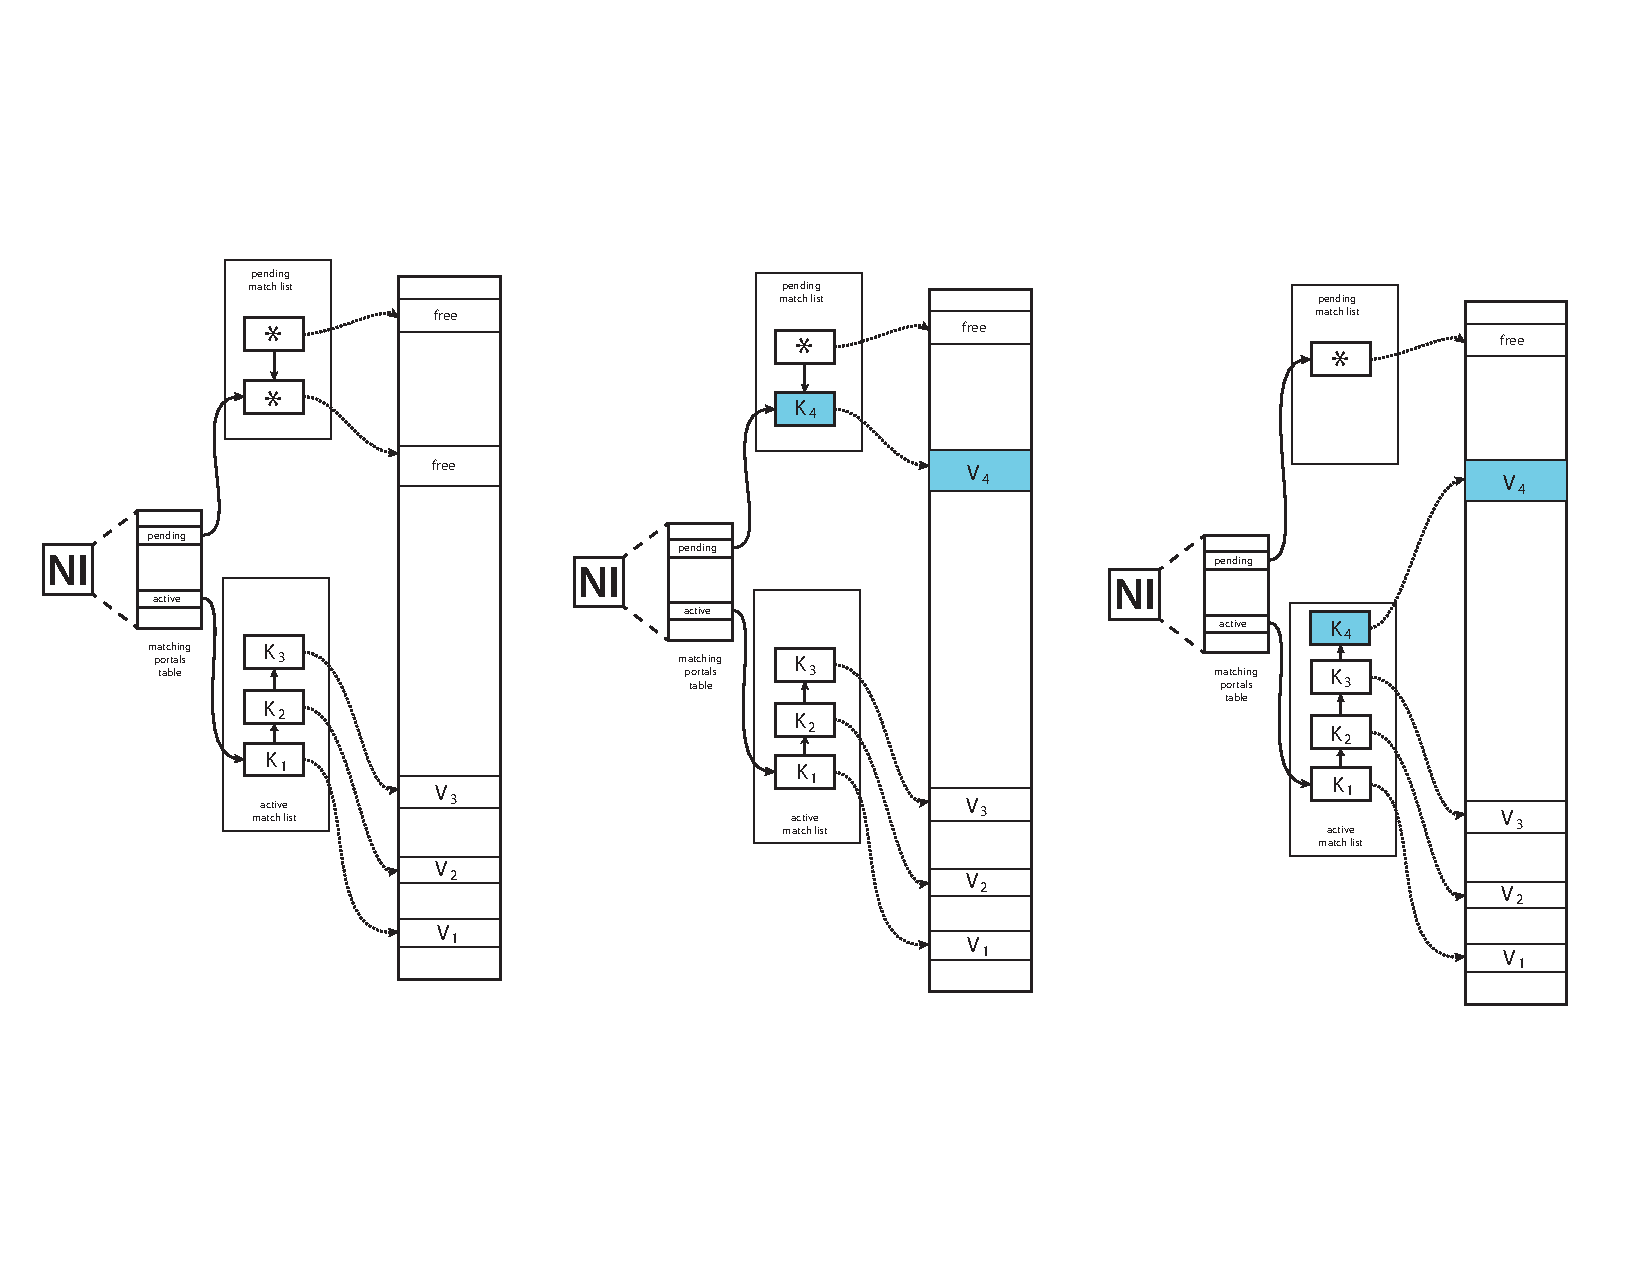
\includegraphics[width=\linewidth]{figs/put}
  \caption{Sequence of target-side actions performed during a \pdht~{\tt insert()} operation.}
  \label{fig:put}
\end{figure*}

The current approach to handle the match list management between the
pending and active lists is to use a dedicated progress thread. This
thread blocks on the event queue associated with the pending PTE,
and is automatically notified by the Portals layer when an insert request
arrives. As insert requests are received, the
progress thread replaces the consumed wildcard ME on the pending list and allocates a
new pending list entry buffer. The thread also creates a new
ME with the appropriate match bits set and appends it to the active
list. Subsequent data access operations will find a match in the active list.

\subsection{Data Access Operations}

One-sided read, write, and atomic update operations are handled by
computing the hash function on the key, then performing corresponding
one-sided Portals get, put, or atomic operation, using the process
rank and match bits provided by the hash. If the operation is unable
to find a matching entry on the active match list, the operation
reports a not-found message. If the key of the retrieved table entry
doesn't match the requested key, \pdht notes the collision and either
returns control to the application or performs a linear probe,
depending on the desired behavior.

\subsection{Collisions and Key Sparsity}

Collisions occur when multiple keys map to the same rank/hash pair.
In the case of a collision,
PDHT utilizes a linear probing solution. The library can
also be configured to simply detect collisions and let the application
take an appropriate action.
% JSD: How does linear probing work?
% DBL:
% pdht_get(key,...): -> 
% while (!found) {
%    PtlGet(match, pte, rank, data, ...)
%    if (data.key != key) { match = match+1; }
% }

A significant difference between traditional hash tables and \pdht is
that using the Portals match list for table entries detaches the link
between the computed hash code and the actual location in
memory. Typically, a hashed key, $K$,  is used with modular arithmetic to
determine a location in an array of size $N$. The hash function
provides a mapping between $|K| \rightarrow N$ elements. When $|K|$ is
much larger than $N$, the likelihood of collisions increases. In order
to manage collisions, hash tables typically store a list of objects within
each array entry.
% JSD: The set of processes sort of takes the place of the array?
% 
% DBL: the set of processes + set of match bits takes place of the array
%
% traditional: hash(key) -> bucket in |0..N-1| -> array[bucket]
%
% pdht: hash(key) -> rank,bits in |NP * 2^64| -> ME
%           each ME -> array[bucket] at creation time via insert or
%           polling thread

\pdht also uses an array to hold the collection of hash table
entries, but the indexing into this array is performed indirectly,
through the ME in the match list. A \pdht hash function provides the 
mapping: $|K| \rightarrow P \times 2^{64}$. Each key is mapped to one
of $P$ distinct process ranks and a unique 64-bit match bits
value. Compared to traditional implementations, $N \ll  P \times
2^{64}$, which has the impact of dramatically reducing the likelihood
of a collision, provided a reasonable hash function.


%%% Local Variables:
%%% mode: latex
%%% TeX-master: "paper"
%%% End:

\section{Experimental Results}

% compare things against polling/triggered
% compare things against matchlist length / hashed Portals / multi-PTEs


%We have gathered preliminary performance results using a prototype
%implementation of \pdht running on the Portals reference
%implementation~\cite{portals-code}. Results were gathered on a cluster system
%part of the Advanced Systems Technology Test Bed at Sandia National
%Laboratories.  The cluster contains 36 compute nodes, constructed with dual
%16-core Intel\regtm Haswell\regtm processors and 128 gigabytes of memory. Nodes
%are connected using a Mellanox\othertm FDR 56Gb/s InfiniBand\othertm fabric.

Performance results were gathered using a prototype implementation of \pdht
running on a version the Portals reference
implementation~\cite{portals-code} that was modified to support the features
presented in Section~\ref{sec:ptl-ext}. Results were gathered on the Comet
cluster
system at the San Diego Supercomputer Center with access provided through the
Extreme Science and Engineering Discovery Environment (XSEDE) program. Comet
contains nodes with several configurations; these experiments were conducted a
portion of the 1944 nodes with Intel\regtm Xeon\regtm E5 processors, comprising
Dell\othertm PowerEdge\othertm C6320 server each with dual 12-core Intel\regtm
Xeon\regtm E5-2680 processors and 128 gigabytes of memory. Nodes are connected
using a Mellanox\othertm FDR 56Gb/s InfiniBand\othertm fabric.

\subsection{Experimental Setup}

To measure the effectiveness of implementing PDHT directly on top of Portals,
we constructed an MPI version of PDHT. The MPI version implements the PDHT
functionality using a companion processes to act as a PDHT server and handle
insertion, access, and update requests.  The MPI PDHT companion process is
implemented using MPI send and receive operations.  It relies on the same hash
function to determine rank and match bits, but internally stores PDHT elements
in an efficient hash table on each local process~\cite{uthash}, keyed with the
same 64-bit value returned by the PDHT hash function. 

%All tests are run using the MPICH 3.2 MPI run-time, configured to use a Portals
%4 channel for all communication operations.

Experiments run with OpenMPI are using version 3.0.0, which has been configured
to use Portals 4 as the message transport layer for all communication
operations. The MPICH MPI tests are run with version 3.2.1 using Portals 4 as
the {\tt ch3} netmod. The MVAPICH2 tests are run with version 2.1 and the
runtime is configured to directly use the InfiniBand\othertm Verbs interface.

One of the primary challenges in deriving performance results for this work is
that the Portals 4 runtime library was developed as an exploratory framework
for modeling next-generation hardware offload network processing. As a result,
Portals message processing is performed by the host processor in a Portals-level companion thread and
incurs higher overheads than would be expected with a hardware accelerated
implementation. Thus, communication performed through the Portals 4 runtime
library has not been optimized as extensively as other high-performance network
middleware (e.g. MVAPICH2). Where possible in our evaluation, we have measured
these overheads and presented comparisons that demonstrate the relative
performance potential of \pdht.

%Results from both native PDHT and MPI-based applications that use the reference implementation are skewed by this
%difference in focus. 

% latency
% need to talk about OpenMPI, PDHT, and mvapich

% match list issues
%  - straight bad
%  - multiple PTE
%  - unordered matching
%  - local search

% scaling
%  MPI communication is more expensive than simple PDHT, matching mvapich2
% performance is good, shows that with lower latency performance would be better


\subsection{Communication Operation Costs}

\begin{figure}
  \centering
  \includegraphics[width=.9\linewidth]{plots/mpilatency}
  \caption{PDHT and MPI Access Latency ($\mu$sec)}
  \label{fig:all-latency}
\end{figure}

\begin{figure}
  \centering
  \includegraphics[width=.9\linewidth]{plots/pdhtlatency}
  \caption{PDHT Access Latencies ($\mu$sec)}
  \label{fig:pdht-latency}
\end{figure}


We start by measuring the read latency of the MPI and Portals PDHT
implementations in a two node configuration with one process per node. As can
different be seen in Figure~\ref{fig:all-latency}, the latency of
the native PDHT implemented directly on Portals is faster than that of the MPI
implementations tested with both MPICH and OpenMPI using Portals communication
channels. This microbenchmark tests the latency with local hash table sizes of a varying
number of items. The MPI PDHT implementation tested with the MVAPICH2 system
outperforms all Portals implementations in a raw performance test. We attribute
this to the different design goals of the two systems as mentioned above. Of
particular note are the greatly increasing latencies for the initial native
PDHT implementation. This is caused by the default $O(N)$ linked-list searching in the
Portals reference implementation. When using the unordered matching option, the
native PDHT access times are flat $O(1)$ over all match list lengths.


Next, we examine the impact of different native PDHT implementation techniques
described in the implementation section. Figure~\ref{fig:pdht-latency} compares
the default version with growing latencies with respect to match list length.
By spreading the key/value entries over multiple Portal table entries (i.e.
multiple match lists), we see that this improves performance, but still causes
latencies to grow as more entries are added. Using the unordered matching
feature in the current version of Portals, we see that PDHT is able to run with
good, flat latencies as the number of local entries increases. Lastly, we see
the impact of searching the local match list rather than performing a full {\tt
  PtlGet()} when fetching entries on the local process rank. This lowers the
access latency by an order of magnitude.

\begin{figure}
    \centering
    \includegraphics[width=.9\linewidth]{plots/scaling1k}
    %\caption{System throughput for a range of local volume (entries per node).}
    \caption{Aggregate system throughput (1K elements).}
    \label{fig:throughput-small}
\end{figure}

\begin{figure}
    \centering
    \includegraphics[width=.9\linewidth]{plots/scaling64}
    %\caption{System throughput for a range of local volume (entries per node).}
    \caption{Aggregate system throughput (64K elements).}
    \label{fig:throughput-big}
\end{figure}

As shown in Figure~\ref{fig:throughput-small}, we measure the weak scaling
of \pdht read operations on the key/value store by examining the
overall throughput of the system. A total of twelve processes are run per node, allowing
additional cores to be used for Portals progress threads or MPI companion processes.  Each process owns a fixed number of
hash table elements that are read by a neighboring process. The
system performs as expected under weak scaling, with overall system
throughput increasing with the number of processes involved. We compare
PDHT native performance against MPI using the MVAPICH2 runtime.

With smaller
entry sizes, we can see that MVAPICH2 performs better than PDHT. 
This performance gap is largely due to the increased latencies when using a
software simulation of Portals on an InfiniBand network. By increasing the size of a key/value entry to
64KB, data transfers become bandwidth bound and the impact of these overheads on performance becomes negligible.
Figure~\ref{fig:throughput-big} shows the convergence in overall system
throughput. Portals-based MPI implementations did not scale favorably with
either native or optimized MPI; thus we do not report results for these implementations because of performance bugs.
%XXX This is where we should do some 
%analysis with round-trip communications in native vs. MPI implementations. It's late.


%To verify this, we measure the performance of retrieving elements from
%the \pdht with respect to the number of elements on each process.
%These results are shown in Figure~\ref{fig:mlen} and provide an
%initial characterization of the lookup cost associated with our \pdht
%implementation.  In contrast with traditional PGAS approaches,
%building a remotely accessible key/value store on top of a mechanism
%intended to support MPI message matching can add new overheads.  In
%particular, the Portals message processing engine must traverse the
%active match list until an ME that matches the given query is located.
%In cases where the element does not exist, the Portals layer must
%reach the end of the list to make this conclusion.  Thus, there is a
%list traversal overhead that is proportional to the number of elements
%visited before finding a match.

Collisions are a source of overhead in any distributed hash table.  This, it
is also useful to explore how the design of the PDHT system can reduce the
number of collisions that occur when compared with  more traditional direct
array-indexed distributed tables. The benchmark code used in another comparison
of UPC, MPI, and SHMEM-based approaches to distributed hash
tables~\cite{maynard:12} was adapted for use with PDHT. This benchmark is
designed to create collision conditions with moderately sized tables. We
compared the OpenSHMEM version of this benchmark against PDHT and found that
with an 80,000 element local table size, the OpenSHMEM implementation had
79,542 collisions for 160,000 insertions. The same set of insertions made with
PDHT resulted in no collisions, due to the indirection provided by the
64-bit match bits as opposed to a direct array index. In practice, we have
not seen collisions in any of the benchmarks described in this section.



% XXX Collisions
%  numbers from SOS vs PDHT benchmark 300K/host

% latency with MPI vs. native
% throughput with MPI vs. native
% matchlist performance
% performance relative OpenSHMEM hash table implementation
% performance of MADNESS reconstruction MPI vs. native
% performance of MADNESS compression MPI vs. native
% performance of MADNESS diff MPI vs. native
% performance of sparse-matrix operation, MPI vs. native




%\subsection{Sparse Matrix Multiplication}
%
%This benchmark application computes the matrix product of two sparse 
%matrices. Matrix sparsity is maintained by decomposing the source
%matrices into tiles containing non-zero and zero elements. Tiles 
%containing non-zero elements are added to the PDHT at the beginning of
%the computation. The matrix multiplication then operates in a SPMD
%fashion with each process requesting the necessary tiles to compute
%the partial product. If either of the operand tiles are not in the
%key/value store, the process continues on until it reaches a tile 
%with non-zero elements. The performance of this benchmark is shown in
%Figures~\ref{fig:4} and \ref{fig:5}.
%
%\begin{figure}
%  \centering
%  \fbox{\rule{2.5in}{0pt}\rule[-2.5in]{0pt}{4ex}}  
%  \caption{Sparse-matrix multiplication weak scaling}
%  \label{fig:4}
%\end{figure}
%
%\begin{figure}
%  \centering
%  \fbox{\rule{2.5in}{0pt}\rule[-2.5in]{0pt}{4ex}}  
%  \caption{Sparse-matrix multiplication strong scaling}
%  \label{fig:5}
%\end{figure}
%


\subsection{MADNESS}

The MADNESS multiresolution numerical computation framework~\cite{thornton09}
has been used to solve a variety of quantum chemistry problems at scale. The
system utilizes wavelet-based functions implemented using 3 to 6 dimensional
spatial representation trees. MADNESS trees represent functions with
coefficients stored in either a scaling basis or a wavelet basis. Certain
operations on the function tree can only be performed in one or the other basis
modes. These spatial decomposition trees are sparse structures, with larger
subtrees corresponding to higher-frequency components of the modeled function.
PDHT can be used to provide a PGLAS system that represents each tree node in
terms of it's spatial coordinates and location (depth) within the tree.

We consider three operations provided by the MADNESS framework. The
first two are conversion operations: {\em compression}, in which scaling
coefficients are converted to the wavelet basis, and {\em reconstruction}, the
complementary operation. The last operation is {\em differentiation}, in which
the derivative of a function tree is computed with respect to a single
dimension. 

\begin{figure}
  \centering
  \includegraphics[width=.75\linewidth]{figs/diff}
  \caption{MADNESS differentiation operation}
  \label{fig:diff}
\end{figure}


The differentiation operation is an irregular operation and is easily expressed
using spatial tree coordinates, but is very difficult using traditional
message-passing (due to tree irregularity) and PGAS (due to physical addressing
requirements). As shown in a Fig.~\ref{fig:diff}a with a 1-D function tree,
taking the derivative at node $i$, requires a convolution with coefficients
from nodes $i-1$ and $i+1$ at the same level within the tree. If these nodes
do not exist, the closest ancestor node must be found and expanded to provide
coefficients at the correct level. 


Figures~\ref{fig:mad-compress}--\ref{fig:mad-diff} show the performance of the
Portals-based PDHT implementation relative to the MPI implementation in a strong
scaling experiment.

\begin{figure}
  \centering
  \includegraphics[width=.9\linewidth]{plots/compress}
  \caption{MADNESS compression performance ($\mu$ sec)}
  \label{fig:mad-compress}
\end{figure}

\begin{figure}
  \centering
  \includegraphics[width=.9\linewidth]{plots/reconstruct}
  \caption{MADNESS reconstruction performance ($\mu$ sec)}
  \label{fig:mad-reconstruct}
\end{figure}


\begin{figure}
  \centering
  \includegraphics[width=.9\linewidth]{plots/diff}
  \caption{MADNESS differentiation performance ($\mu$ sec)}
  \label{fig:mad-diff}
\end{figure}

\subsection{Meraculous}

The NERSC Meraculous benchmark performs de novo whole genome assembly,
reconstructing genomic sequences from overlapping and erroneous fragments
produced by a high-throughput sequencer. Meraculous constructs a graph of all
overlapping substrings in the input and traverses the graph to discover all
linear subgraphs. These subgraphs correspond to contiguous sequences of
genomic data. Meraculous is written in UPC and uses a hash table
to represent the de Bruijn graph. 

We have adapted the Meraculous benchmark~\cite{georganas:14} to store the de Bruijn
graph using \pdht instead of a UPC hash table. Both structures utilize the same key
structure and creation algorithm. The graph traversal is performed in parallel
by iterating through all local entries in the table and walking both the left
and right ends of the sequence. The results of this experiment are shown in
Figure~\ref{fig:meraculous}. The input file for this experiment was the {\tt
  human-chr14.txt.ufx.bin} data set available as a part of the NERSC benchmark
suite. This input set consists of 96 million sequences, each of which must have
an ME in Portals. At small scale, this consumes a much greater number of
Portals resources than is typically supported. On the other end, adding 
processes reduces Portals resources, but runs out of work quickly.

\begin{figure}
  \centering
  %\fbox{\rule{2.5in}{0pt}\rule[-2.5in]{0pt}{4ex}}  
  \includegraphics[width=.9\linewidth]{plots/meraculous}
  \caption{Meraculous UPC vs PDHT performance($\mu$ sec)}
  \label{fig:meraculous}
\end{figure}


%%% Local Variables:
%%% mode: latex
%%% TeX-master: "paper"
%%% End:

\section{Related Work}

\cite{fompi13,cmpi10,mht15}
\cite{prefix04,chord01,kademlia02,pastry01,memcached04}
\cite{zht13}
\cite{memcached12}

\section{Conclusion}

Capture contributions

Discussion and Future work

%%% Local Variables:
%%% mode: latex
%%% TeX-master: "paper"
%%% End:


%\singlespacing
\bibliographystyle{IEEEtran}
%\bibliography{IEEEfull,refs,dsmbiblio}
%\input{appendix}
\end{document}
